%% ======================================================================
%% FRONTMATTER
%% ⚑ Purpose: pre-content (roman page numbers, unnumbered chapters)
%% ======================================================================
\sloppy % Prevent overfull lines
\frontmatter

% --- COVER PAGE ---
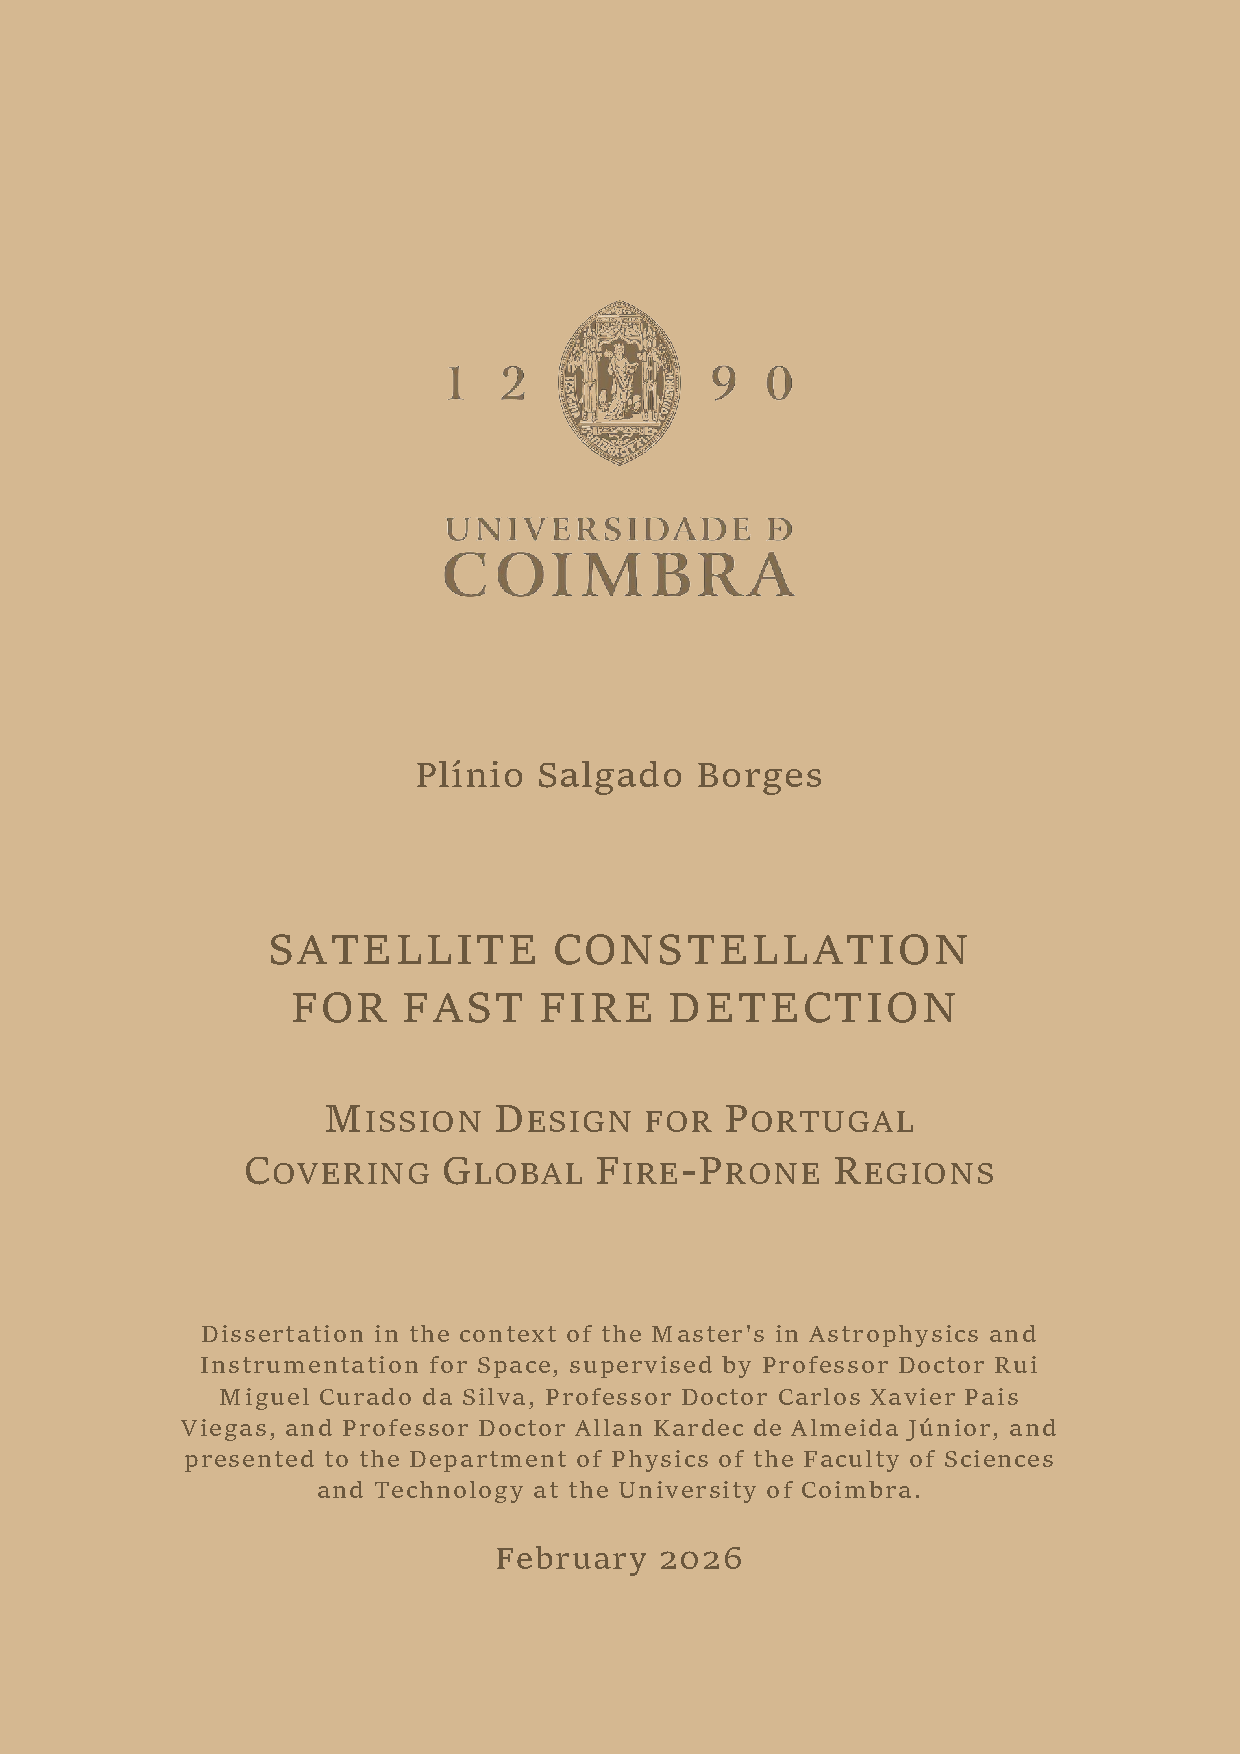
\includepdf[pages={-},pagecommand={}]{images/cover.pdf}
\newpage\thispagestyle{empty}

%\pagestyle{plain}

% --- TITLE PAGE ---
\begin{titlepage}
    \begin{center}
    % UC logo, no name
    
\includegraphics[width=0.34\textwidth]{images/UC_logos/UC_V_FundoClaro-negro.png}
    
    \vspace{0.2cm}
    {\huge{\myname\par}}
    
    % Thesis name
    \vspace{0.3cm}
    {\Huge{\textbf{\thesistitle}}\par}
    
    % Thesis subtitle
    \vspace{0.25cm}
    {\huge{\textsc{\thesissubtitle}}\par}

    \vspace{0.6cm}
    {\normalsize{\textbf{Supervisor:}\\{\supervisorname}\par}}
    
    \vspace{0.3cm}
    {\normalsize{\textbf{Co-Supervisors:}\\{\cosupervisorname}}}
    
    \vspace{0.4cm}
    {\footnotesize{\textbf{Jury:}\\[3pt]
    % TODO: Update jury member names here. This is a manual list.
    Prof.\ Dr. Jury Member 1\\
    Prof.\ Dr. Jury Member 2\\
    Prof.\ Dr. Jury Member 3\\
    Prof.\ Dr. Jury Member 4
    }}
    
    \vspace{0.5cm}
    {\footnotesize{Dissertation submitted in partial fulfillment for the\\degree of Master of Science in Astrophysics\\and Space Instrumentation.}}
    
    \vspace{0.2cm}
    {\small \statedate\par}    
    
    \end{center}
\end{titlepage}

% --- ACKNOWLEDGMENTS ---
\chapter*{Acknowledgments}
\addcontentsline{toc}{chapter}{Acknowledgements}
% ------------------------------------------------------------------
% Acknowledgements
% ------------------------------------------------------------------

% §1 — Institutional Support
% This work was partially funded by the Fundação para a Ciência e a Tecnologia (FCT), I.P., and developed at the Department of Physics of the University of Coimbra.

% §1b — Personal arc
This work grows out of a journey that began when, as a teenager in Brazil, I observed the planets through a telescope I had built with my own hands---deciding then to become a physicist. I started my studies at Brazil (UFMG) in 2010, spent time in Coimbra in 2011, and in Germany 2014, on this track specizlized in precision optics, working on systems ranging from Alzheimer's disease detectors to optical calibration of satellites (Sentinel-5). That path brought me back to Coimbra, more than a decade later, to complete the Master's in Astrophysics and Space Instrumentation (MAIE) that I had first glimpsed in 2011. Along that journey I witnessed the growing severity of wildfires in both Brazil and Portugal, and chose to dedicate this thesis to a problem that connects the two countries where I have built my life---and the planet I admire. To all who were part of this path---and who allowed me to move from someone who observes other planets to someone capable of conceiving missions to observe and protect the Earth---my most sincere gratitude.

% §2 — Supervisors
Among all, special recognition is owed to my supervisors, whose scientific guidance, intellectual rigour, and constant availability were decisive for the completion of this work.

To Professor Dr. Rui Miguel Curado da Silva, whose expertise in space systems made it possible to transform an initial idea---``Portugal faces wildfires; how can space instrumentation help?''---into a structured mission, connected to wildfire combat groups (ADAI) and to CubeSat fire-detection projects (FADO\footnote{F.A.D.O -- Fire Analysis \& Development Observatory, Concept Report CubeSat 2024, Team CSP-7-FADO.}), in which I participated and from whose colleagues I learned a great deal. His teaching in the space instrumentation course was essential for building the knowledge required to start this work, and his ability to connect people and institutions within the Portuguese space ecosystem was instrumental in defining the directions of this thesis and the future paths for fire-detection sensor development.

To Professor Dr. Carlos Xavier Paes Lidas, whose expertise in wildfire management and combat technologies---namely fire-spread modelling and the use of satellite imagery by firefighting authorities in Portugal---was fundamental in defining what the mission had to fulfil in the context of fire detection in Portugal. Part of the knowledge and data that informed this thesis was derived from two projects connected to Professor Carlos: the project IMFire---Intelligent Management of Wildfires\footnote{This work was carried out under the project IMFire---Intelligent Management of Wildfires, ref.\ PCIF/SSI/0151/2018, partially funded by national funds through the Ministry of Science, Technology and Higher Education, Portugal.}, and the project ForestSphere\footnote{This research was partially funded under the Protocol between Fundação para a Ciência e a Tecnologia and the Agency for Administrative Modernization, I.P.\ (AMA), through the project ForestSphere, ref.\ 2025.01496.DT4ST.}. It was also he who introduced me to Professor João Luís Ruivo Carvalho Paulo and the artificial-intelligence-based fire detection work within the FireSys project.

To Professor Dr. Alan Kardec de Almeida Júnior, whose knowledge of orbital mechanics was essential for advancing from basic mission requirements to high-fidelity models. He taught me to use GMAT, the mission-analysis tool developed at agencies such as NASA, and transmitted to me the fundamentals of celestial mechanics, perturbation forces, atmospheric drag, orbital stability, station-keeping, and the simulation tools required---foundations that constitute the simulation infrastructure presented here. I am equally grateful for his careful guidance in the writing and revision of this work.

To all three, my most sincere gratitude for the support, encouragement, and trust throughout this journey.

% §3 — Project Collaborators
I am equally grateful to Professor João Luís Ruivo Carvalho Paulo for the opportunity to work on the FireSys\footnote{This dissertation work was partially supported by the project FireSys -- ``Intelligent Decision Support System for Management of Wildfires'' with reference of operation 21378, operation code COMPETE2030-FEDER-02230700 on Balcão dos Fundos, funded by the Fundo Europeu de Desenvolvimento Regional (FEDER), through the Innovation and Digital Transition Program (COMPETE 2030) of Portugal 2030.} project on satellite-image-based fire detection using AI. From that project emerged the \emph{Watcher--Zoom} concept presented in this work.
I thank colleagues PhD\,(c) Dina Jahanianfard, who shared valuable insights on satellite image processing related to Sentinel-2 and the demonstration of the \emph{Watcher--Zoom} concept, and PhD\,(c) Matheus Fernandes Kovaleski, who collaborated on the code development.
I thank Dr.\ Timothée Vaillant for his suggestions regarding the defence presentation.
I also wish to thank the MAIE coordinators: Prof.\ Dr.\ Margarida Maria Lopes da Silva Camarinha, whose teaching in the Celestial Mechanics course provided the mathematical foundations and formalism present in this work, and Prof.\ Dr.\ Alexandre C. M. Correia for his support in navigating the decisions that helped define the thesis topic during the Master's and in bringing this work to completion.

% §4 — Scientific and Professional Formation
It is also important to acknowledge the experiences that built the foundations of this work before I arrived in Coimbra, starting in Brazil at UFMG. To Professor Dr. Ado Jório Vasconcelos, for the scientific training in optics at LabNS that constitutes my technical base and for believing in me at the start of my career, and to Professor Dr. Leandro Malard and colleagues at LabNS for their contributions to that formative in a unique environment. To Professor Renato Las Casas at the Observatório da Serra da Piedade, who taught me how to share the sky with others, and to Bernardo Riedel, who taught me the art of building telescopes. To Dr.\ Luiz Etrusco and colleagues at InventVision, for their support during my studies and in the development of advanced cameras. To Dr. Ivo Vieria and colleagues at LusoSpace, for showing me in practice how space systems are built.

% §5 — Colleagues and Friends
I wish to thank all the friends and colleagues who were with me at the University of Coimbra or who were part of this journey to the completion of the Master's, and who at the right moments helped me to relax, enjoy nature, and reflect on ideas.
To Flávia Amaral, astrophysicist and friend who can see vast distances in the universe that I can only begin to imagine, and who has accompanied this journey since 2010 at UFMG. To Pedro Pessoa, mathematician and friend whose mastery of geometry in many dimensions accompanied and enriched our studies in general relativity.
To my Master's friends though this journey ---Cláudia, Letícia, Snock, Aline, Guilherme, Carlos, João Werneck, Akel, Céci, Willian, Ronald, Rita, José Rodrigues, Fred, Maria João, Ricardo, Mariana Encarnação, Inês de Castro, Maria Campino, Fernanda, Joana, Cátia, Hortence, Diogo, Marcos, Angela, and Rubens Silva, Thiago Célio, Thiago Duarte, Filomeno, Eduardo Valadares, Ubirajará Agero, Paula, Renan, Alexandre, Emerson, Fabiano, Marcia, Hudson, Caciano, Lucas, Aroldo, Luiz, Wescley, Camila, Marina, Paola, Bruno, Erlan, André, Rafael, Luis, Kenji, André, Beto.
A special thank-you to Lara and Fig, for showing me that my technical skills in optical instrumentation, combined with space systems, could have a real impact on climate challenges---revealing a meaningful professional path, with consequences for the lives of many people and beings on this planet, and influencing the choice of the topic of this thesis.

% §6 — Family
Finally, I wish to express my deepest gratitude to my family.
To my father Joel and my mother Marisa, who supported me unconditionally at every stage---from the education they provided in Brazil to the decision to study abroad---and who, even at a distance, were never absent.
To my sisters Sabrina, Mariana, and Marina, for their constant encouragement and for always reminding me of what matters.
To all members of the family who contributed, throughout my life, with support, guidance, and the example that sustained effort is the surest way to accompanying our dreams.
This work is also yours.


% --- ABSTRACTS ---
\chapter*{Abstract}
\addcontentsline{toc}{chapter}{Abstract}
Lengthening fire-weather seasons and shifting vegetation flammability are driving unprecedented fire activity across Mediterranean Europe and other fire-prone regions. Portugal exemplifies this trend: extreme fire-weather indices have risen steadily since the late twentieth century, and projections indicate the most severe fire-weather class will cover much of the country by mid-century. Effective fire management demands rapid detection at scales fine enough to resolve individual fire fronts, yet no current or planned satellite system delivers both sub-hour revisit and metre-class resolution where it is needed most.

Geostationary sensors scan continental areas every 10--15~minutes but resolve only 2--3~km per pixel, while low-Earth-orbit missions achieve sub-30~m resolution at the cost of multi-day revisit intervals. This resolution--revisit--latency gap leaves fire-prone territories without timely, high-resolution space-based fire intelligence. The present work asks: \emph{What constellation design can close this gap, achieving roughly 30-minute revisit and approximately 6~m ground resolution over continental Portugal?} A secondary question is: \emph{What coverage does the constellation provide over global fire-prone regions?}

The study integrates fire-remote-sensing science, orbital mechanics, and high-fidelity numerical simulation.
A core study domain was first delineated by to Portugal's territory according it's fire season pattern, than a global study domain was defined to current fire-weather severity, establishing the geographical, spatial, and temporal requirements the constellation must satisfy.
An analytical survey of repeating ground-track orbits (RGTOs), generalised to arbitrary target latitudes, produced a family of RGTO modes for daily revisit in continental Portugal; from this group of orbital geometries the ratio $\tau = 15/1$ at approximately 488~km altitude and inclination ${\sim}\,40.2°$~was selected as best matched to the target latitude core study domain at center of Portugal, an resonating orbit around the city of Coimbra, providing the fastest revisit possible.
This selected orbitalmode was embedded in a Walker constellation framework. Parametric trades then explored the number of orbital planes, satellites per plane, and maximum sensor off-nadir viewing angle within a Walker-delta framework were allowed to optmized the revisit over the Portuguese core study domain.
The candidate constellations were propagated sing the high-fidelity General Mission Analysis Tool (GMAT) --- with a $8\times8$ geopotential, lunisolar perturbations, and atmospheric drag--- validating the orbital stability, observational-link pattern, temporal coverage, revisit statistics, and ground sampling distance over both the Portuguese core domain and a global fire-prone domain. 

The selected constellation---designated $C_{\text{Zoom}} = C_{15/5/72}$, comprising 15~satellites in 5~equally spaced orbital planes phased by $72^\circ$ of right ascending node, with 3 satellite per plane distributed $120^\circ$ of each by shifts in the true anomaly---achieves a mean revisit of approximately 21~minutes over Portugal with ground resolution below 6~m per pixel.
The repeating ground-track design delivers roughly $1.75\times$ the daily coverage time of a conventional sun-synchronous orbit at comparable altitude, effectively halving the fleet size that would otherwise be required.
A sensitivity analysis confirms that a $65°$ off-nadir sensor limit is essential: tightening it to cover only Portugal $30°$ keeping same cadence nearly doubles the required fleet to 27~satellites, underscoring wide-angle pointing as a key design driver for keeping the constellation compact.
Designed for Portugal, the coverage footprint extends naturally to all major fire-prone regions with exception of boreal region: the temperate belt---California, the broader Mediterranean basin, southern Africa, and south-eastern Australia---receives 6--7~hours of daily observation with worst-case revisit gaps of about 30 minutes, while tropical regions such as Amazonia, central Africa, and south-east Asia retain at least 3.5~hours per day with an average revisit around 40 to 50 minutes.
To expand the narrow field of view that metre-class resolution demands on a small platform, a \emph{Watcher--Zoom} tip-and-cue architecture is proposed: five existing geostationary fire-detection satellites provide coarse alerts every 10--15~minutes, cueing the nearest low-orbit spacecraft to steer its imager toward the hotspot and acquire high-resolution imagery.

No surveyed fire-detection constellation combines sub-30-minute revisit with metre-scale resolution over any examined fire-prone region. The architecture proposed here---fifteen satellites on a resonant orbit, guided by geostationary fire-watch assets---closes this gap for Portugal and extends meaningful coverage to every major fire-prone region on Earth, turning a national mission into a global cooperative-observation platform.


The study integrates fire-remote-sensing science, orbital mechanics, and high-fidelity numerical simulation. A core study domain was delineated over Portugal according to its fire-season pattern; a global domain was then defined by current fire-weather severity, establishing the geographical, spatial, and temporal requirements. An analytical survey of repeating ground-track orbits (RGTOs), generalised to arbitrary target latitudes, produced a family of modes for daily revisit over Portugal; from this set the ratio $\tau = 15/1$ at approximately 488~km altitude and ${\sim}\,40.2°$ inclination was selected as best matched to the core domain centred on Coimbra, providing the fastest revisit. This orbital mode was embedded in a Walker-delta framework; parametric trades explored the number of planes, satellites per plane, and maximum off-nadir angle to optimise revisit. Candidate constellations were propagated with the General Mission Analysis Tool (GMAT)---$8\times8$ geopotential, lunisolar perturbations, and atmospheric drag---validating orbital stability, coverage, revisit statistics, and ground sampling distance over both domains.

The selected constellation---$C_{\text{Zoom}} = C_{15/5/72}$, 15~satellites in 5~planes phased by $72^\circ$, 3~per plane at $120^\circ$ true-anomaly spacing---achieves a mean revisit of approximately 21~minutes over Portugal with ground resolution below 6~m. The repeating ground-track delivers roughly $1.75\times$ the daily coverage of a sun-synchronous orbit at comparable altitude, effectively halving the required fleet. A sensitivity analysis confirms that the $65°$ off-nadir limit is essential: tightening it to $30°$ nearly doubles the fleet to 27~satellites, underscoring wide-angle pointing as a key design driver. The coverage extends naturally to all major fire-prone regions except the boreal belt: temperate zones---California, the broader Mediterranean, southern Africa, south-eastern Australia---receive 6--7~hours of daily observation with worst-case gaps of about 30~minutes, while tropical regions retain at least 3.5~hours per day with average revisit of 40--50~minutes. To compensate the narrow field of view that metre-class resolution demands, a \emph{Watcher--Zoom} tip-and-cue architecture is proposed: five geostationary fire-detection satellites provide alerts every 10--15~minutes, cueing the nearest low-orbit spacecraft to image the hotspot at high resolution.

% \vspace{1em}
% \noindent\textbf{Keywords:} satellite constellation, fire detection, repeating ground-track orbit, mission design, fire detection, Portugal, Earth observation

% --- INSPIRATIONAL QUOTE ---
\chapter*{}
\setlength\epigraphwidth{14.5cm}
\setlength\epigraphrule{0pt}
\makeatletter
\patchcmd{\epigraph}{\@epitext{#1}}{\itshape\@epitext{#1}}{} {}
\makeatother
\vspace*{\fill}
\epigraph{%
\footnotesize\upshape%
February 14, 1990.\\[\medskipamount]
Beyond the orbit of Neptune,\\
after a last encounter with Saturn,\\
Voyager~1 turned its camera homeward\\
and captured the whole of Earth\\
as a single dot, a speck of light.%
\par\medskip \medskip
``From this distant vantage point, the Earth might not seem of any particular interest. But for us, it's different. Consider again that dot. That's here. That's home. That's us. On it everyone you love, everyone you know, everyone you ever heard of, every human being who ever was, lived out their lives.
[\ldots] Our planet is a lonely speck in the great enveloping cosmic dark. In our obscurity, in all this vastness, there is no hint that help will come from elsewhere to save us from ourselves. The Earth is the only world known so far to harbor life. There is nowhere else, at least in the near future, to which our species could migrate.
[\ldots] To me, it underscores our responsibility to deal more kindly with one another, and to preserve and cherish the pale blue dot, the only home we've ever known.''}{Carl Sagan, \textit{Pale Blue Dot} (1994)}
\vspace*{\fill}

%% --- TABLE OF CONTENTS AND LISTS ---
\pagestyle{plain}
\tableofcontents

% \chapter*{List of Acronyms}
%\addcontentsline{toc}{chapter}{List of Acronyms}
% % TODO: Define your acronyms here.
% Use the format: \acro{ACRONYM}{Full Name}
% Then, use \ac{ACRONYM} in your text.
% The first use will expand the acronym, and subsequent uses will show the acronym only.
\begin{acronym}[UC]
    \acro{UC}{University of Coimbra}
    \acro{MSc}{Master of Science}
\end{acronym}

% Example usage to ensure acronym is defined
% \ac{DEA}

\listoffigures
\listoftables

% ── List of FIXMEs (remove before final submission) ──
\listoffixmes